\documentclass[11pt]{ctexart}

\usepackage{geometry}
\geometry{a4paper, margin=2.5cm}
\usepackage{hyperref}
\usepackage{enumitem}
\usepackage{longtable}
\usepackage{array}
\usepackage{graphicx}
\usepackage{float}
\usepackage{xcolor}
\usepackage{titlesec}

\title{Snooker2D 项目结题总结报告}
\author{鲁亦智，何广一，井淳 \quad 台球组}
\date{2026年7月18日}

\begin{document}

\sloppy

\maketitle

\tableofcontents
\newpage

% ============================================================
\section{项目概况}
% ============================================================

Snooker2D 是一个基于 C++17 和 Qt 6 的 2D 斯诺克台球游戏，采用 MVVM 架构，由三名开发者协作完成。项目历经三轮架构重构，从最初的 GameUiBus 中间件方案逐步收敛到 App 层集中绑定的最终形态。相比中期节点，结题阶段新增了加塞（English/Spin）物理系统、中英双语界面、库边预瞄辅助线、GameControlPanel 设置面板、覆盖全部五层的单元测试体系，以及 GitHub Actions CI/CD 自动化流水线。

项目仓库地址：\url{https://github.com/LOnion1124/Snooker2D}。

\begin{table}[H]
\centering
\begin{tabular}{|l|l|}
\hline
\textbf{项目属性} & \textbf{描述} \\
\hline
语言标准 & C++17 \\
UI 框架  & Qt 6 (Widgets) \\
构建系统 & CMake 3.20+ / Ninja \\
包管理   & vcpkg / aqtinstall \\
架构模式 & MVVM（Model-View-ViewModel） \\
编译目标 & 5 层（Common / Model / ViewModel / View / App） \\
测试框架 & 自研轻量宏 + Qt Test + QSignalSpy \\
架构护栏 & PowerShell 脚本 + CMake custom target \\
\hline
\end{tabular}
\caption{项目基本信息}
\end{table}

% ============================================================
\section{技术架构}
% ============================================================

\subsection{分层设计}

项目拆分为五层编译目标，App 层在主可执行文件中完成装配：

\begin{table}[H]
\centering
\begin{tabular}{|c|l|l|l|}
\hline
\textbf{层} & \textbf{职责} & \textbf{编译依赖} \\
\hline
Common     & 全局类型、常量、工具函数、DTO       & 无                       \\
Model      & 游戏状态机、物理引擎、规则判定     & Common + Qt::Core      \\
ViewModel  & 数据翻译、状态推送、命令处理       & Model + Common + Qt::Core \\
View       & 界面渲染、用户输入                 & Common + Qt::Widgets    \\
App        & 对象装配、信号槽绑定               & 所有层                   \\
\hline
\end{tabular}
\caption{五层架构概览}
\end{table}

\textbf{约束}：View 层不链接 ViewModel/Model（CMake 编译期强制），ViewModel 不链接 View。所有跨层信号槽绑定集中在 App.cpp（13 条 connect），配合 ViewModel 构造中的 9 条通知绑定，共 22 条跨层连接。

\subsection{层间通信}

\begin{table}[H]
\centering
\begin{tabular}{|c|c|c|c|}
\hline
\textbf{绑定类型} & \textbf{方向} & \textbf{连接位置} & \textbf{数量} \\
\hline
属性绑定 & ViewModel → View & App.cpp & 6 条 \\
命令绑定 & View → ViewModel & App.cpp & 6 条 \\
视图间绑定 & View → View & App.cpp & 1 条 \\
通知绑定 & Model → ViewModel & ViewModel 构造函数 & 9 条 \\
\hline
\end{tabular}
\caption{信号槽绑定分类}
\end{table}

\subsection{架构演进}

项目经历了三轮架构重构才收敛到最终形态：

\begin{enumerate}[leftmargin=*]
\item \textbf{第一轮}：引入 contracts 层（GameUiBus）和 GameSessionViewModel，View 不再依赖 ViewModel/Model。
\item \textbf{第二轮}：删除 3 个子 ViewModel（GameViewModel / CueControlViewModel / ScoreViewModel），全部合并到 GameSessionViewModel，减少 ViewModel 内部转发。
\item \textbf{第三轮}：取消 GameUiBus，各层自管 signal/slot 声明，App 层集中 connect。当前方案编译依赖由 CMake 强制执行，架构护栏脚本持续验证边界。
\end{enumerate}

% ============================================================
\section{项目成果展示}
% ============================================================

\subsection{游戏主界面}

\begin{figure}[H]
\centering
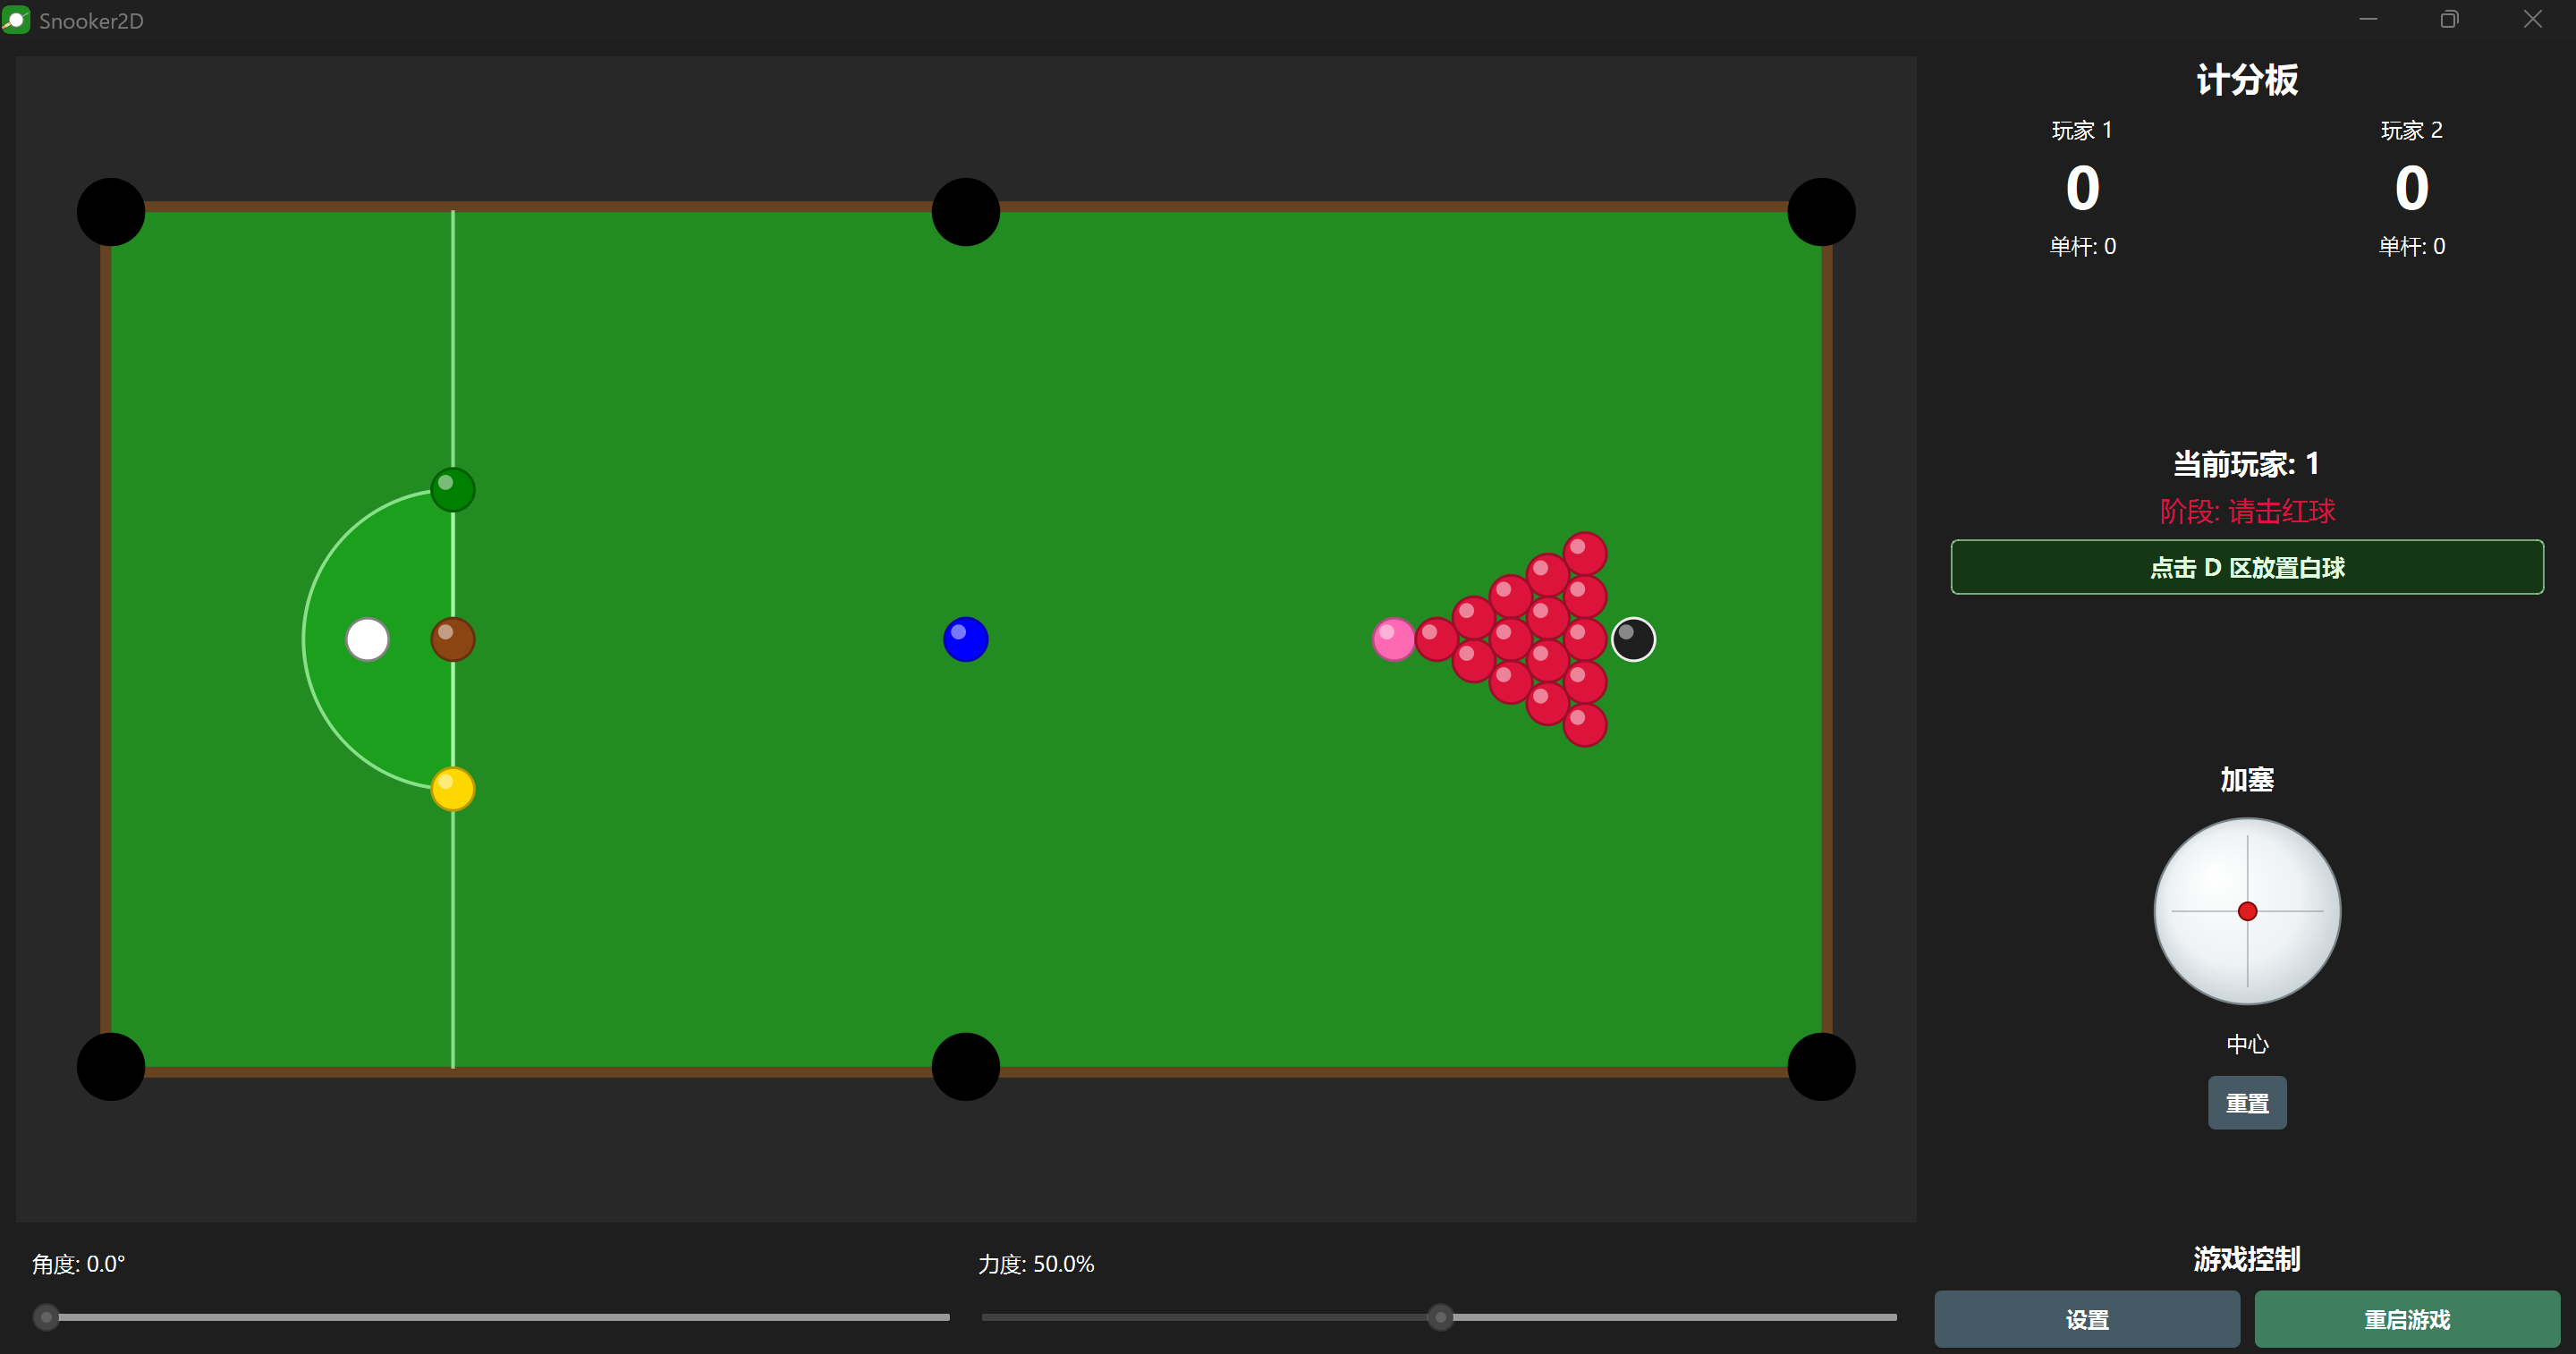
\includegraphics[width=0.85\textwidth]{imgs/main_window.png}
\caption{Snooker2D 游戏主窗口}
\end{figure}

\subsection{物理碰撞与加塞效果}

\begin{figure}[H]
\centering
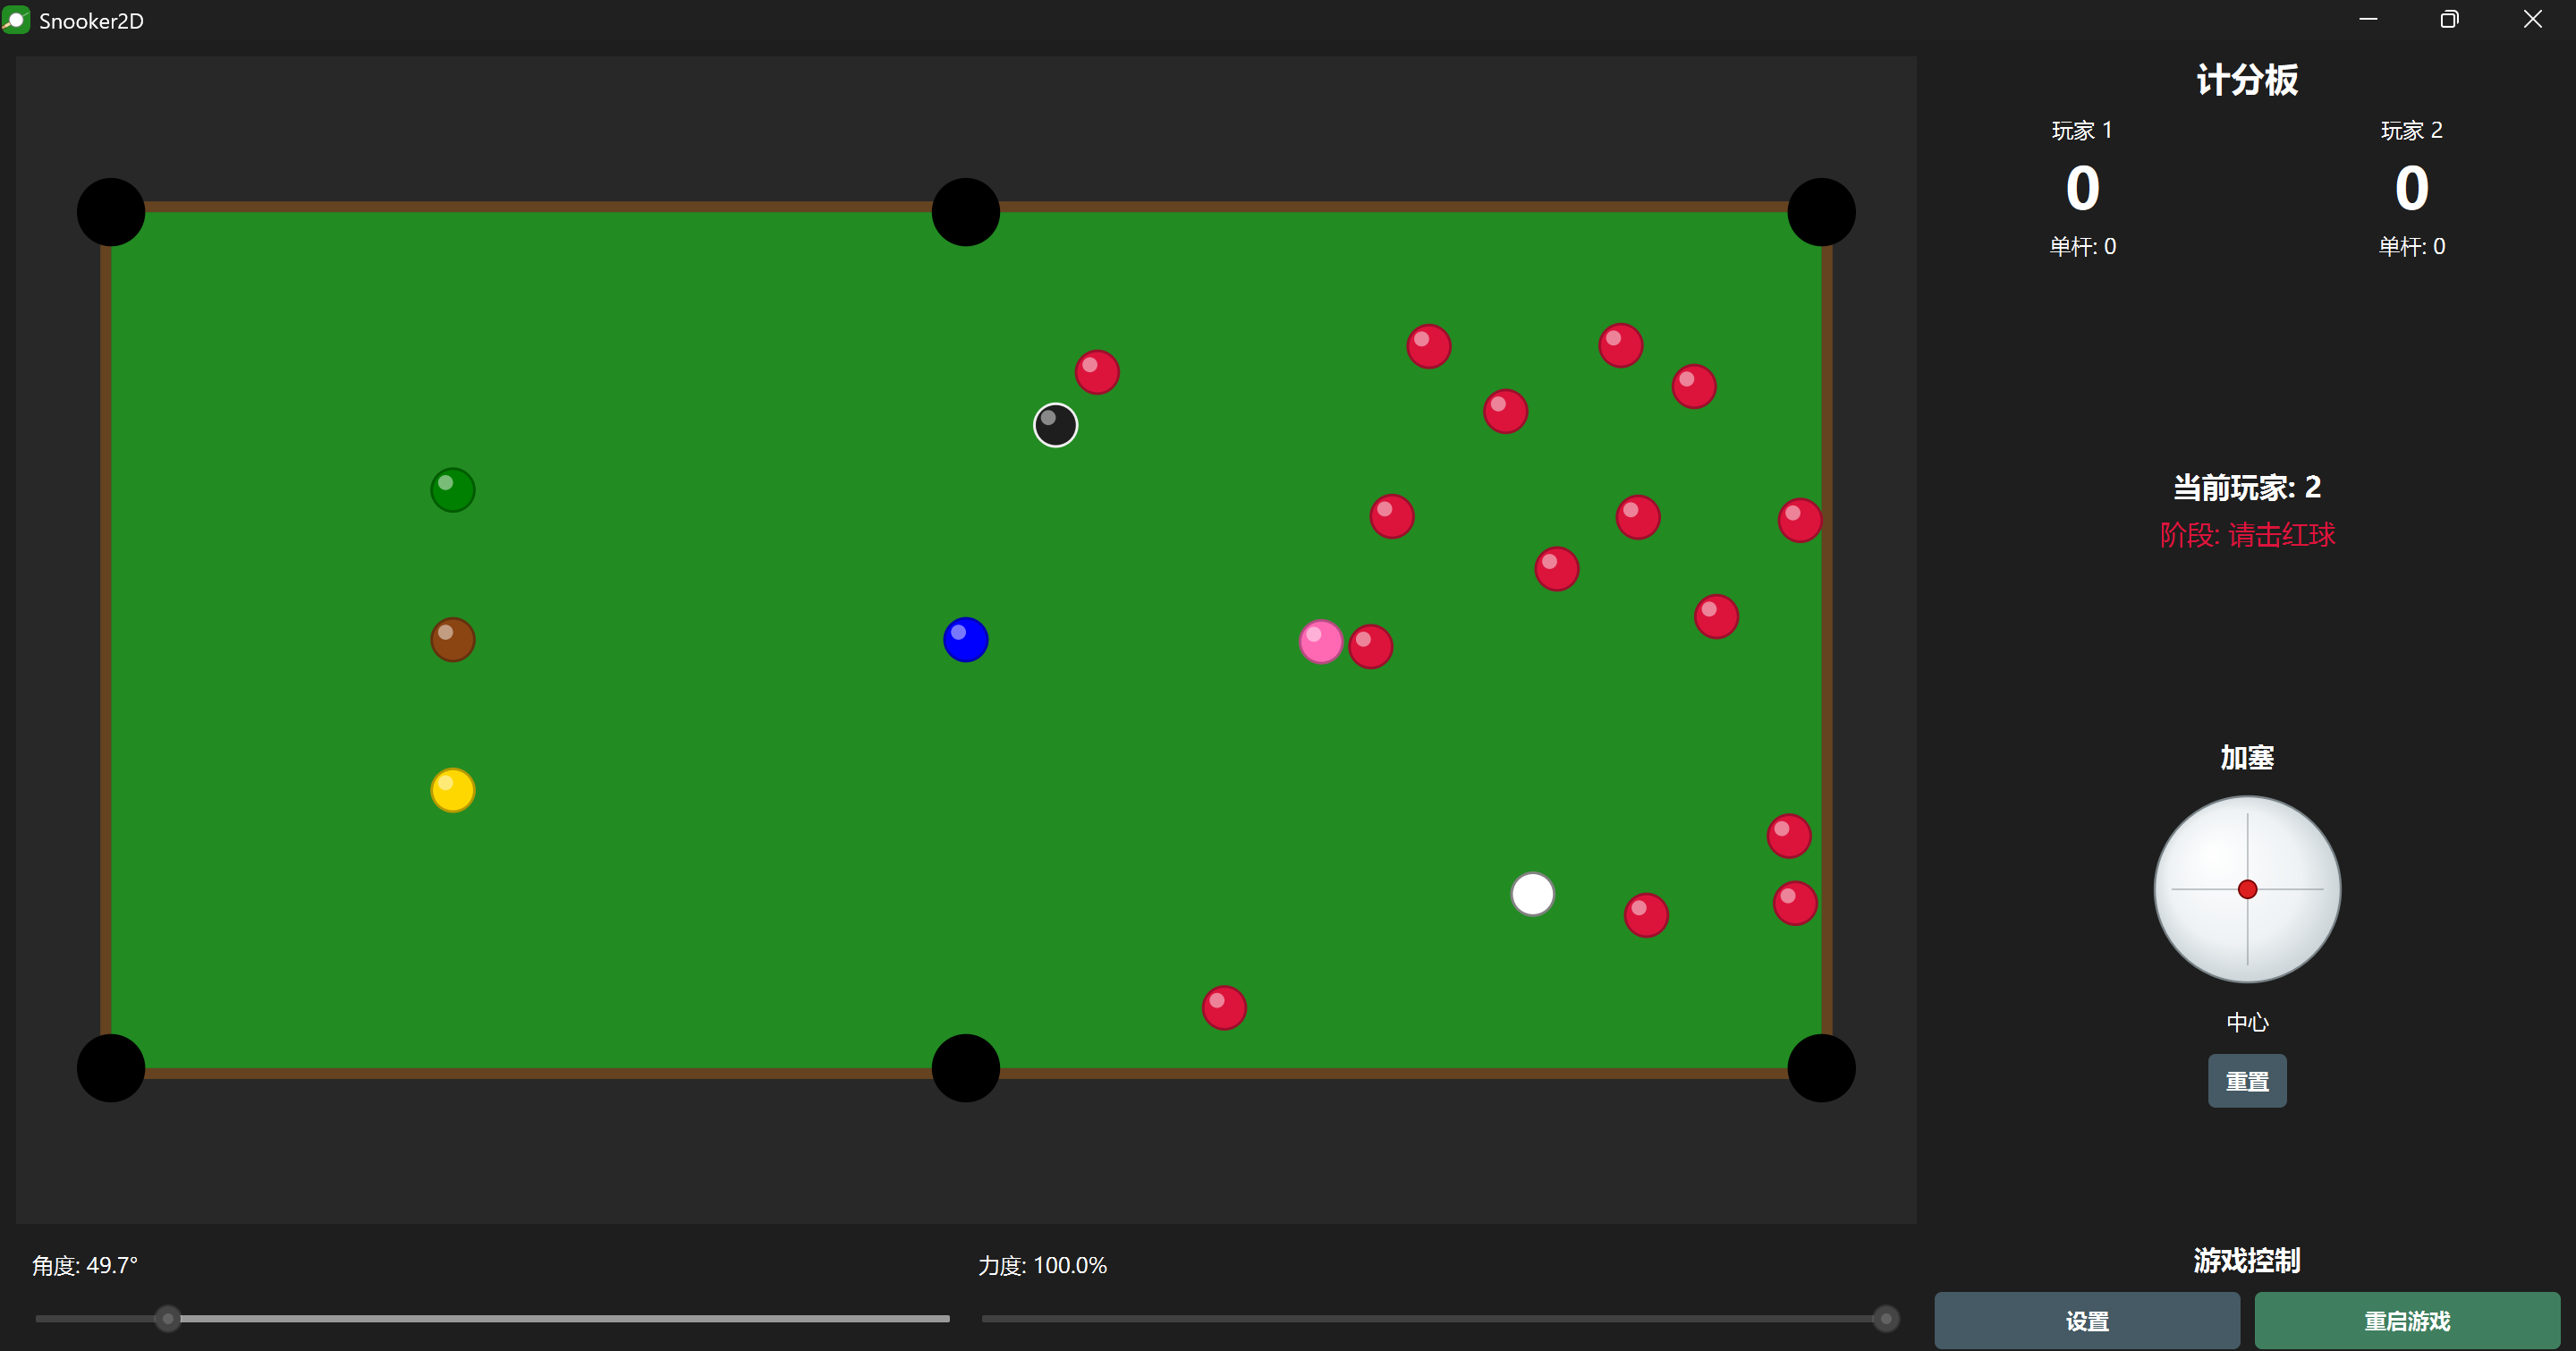
\includegraphics[width=0.85\textwidth]{imgs/physics_collision.png}
\caption{物理碰撞与加塞效果}
\end{figure}

\subsection{D 区白球放置}

\begin{figure}[H]
\centering
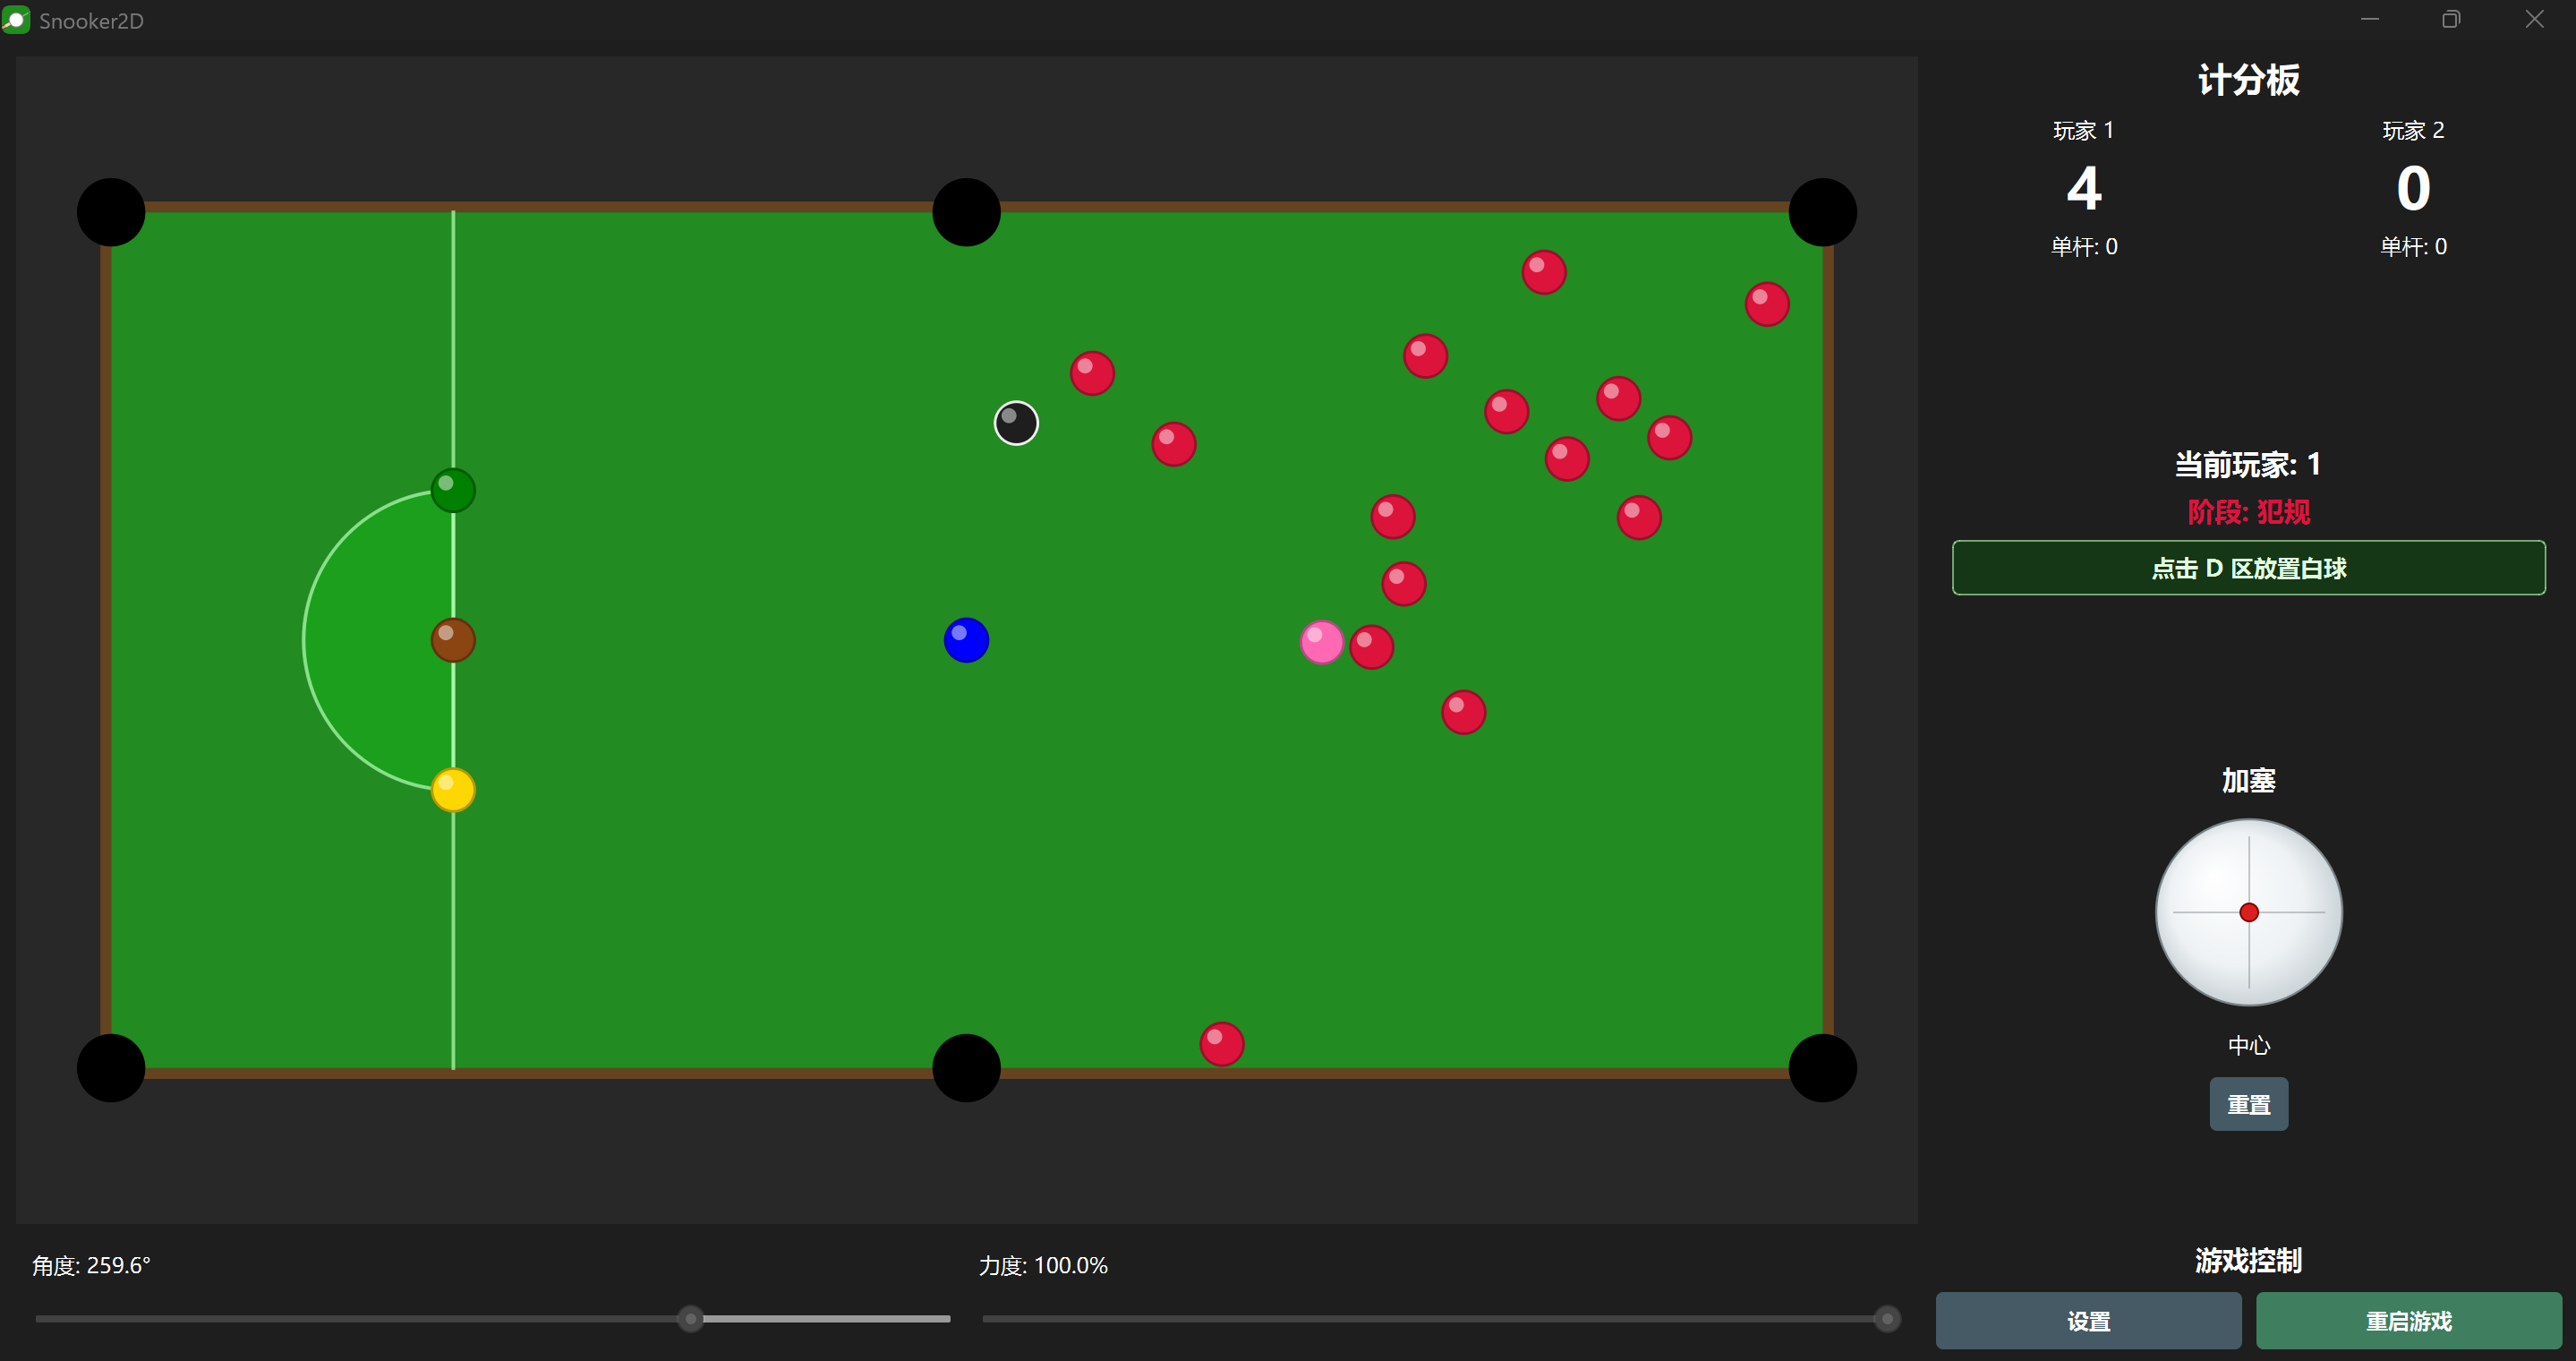
\includegraphics[width=0.85\textwidth]{imgs/place_ball.png}
\caption{D 区白球复位}
\end{figure}

\subsection{其他功能截图}

\begin{figure}[H]
\centering
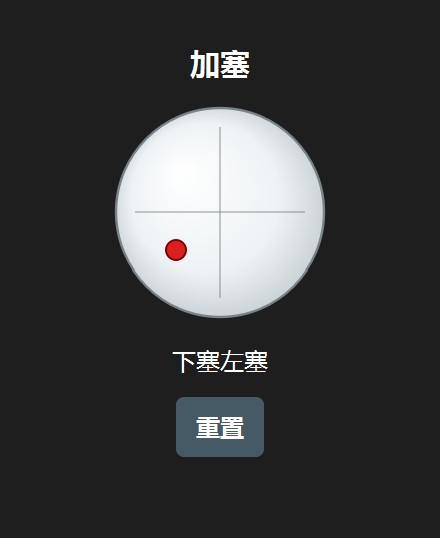
\includegraphics[width=0.75\textwidth]{imgs/english_panel.png}
\caption{加塞控制面板}
\end{figure}

\begin{figure}[H]
\centering
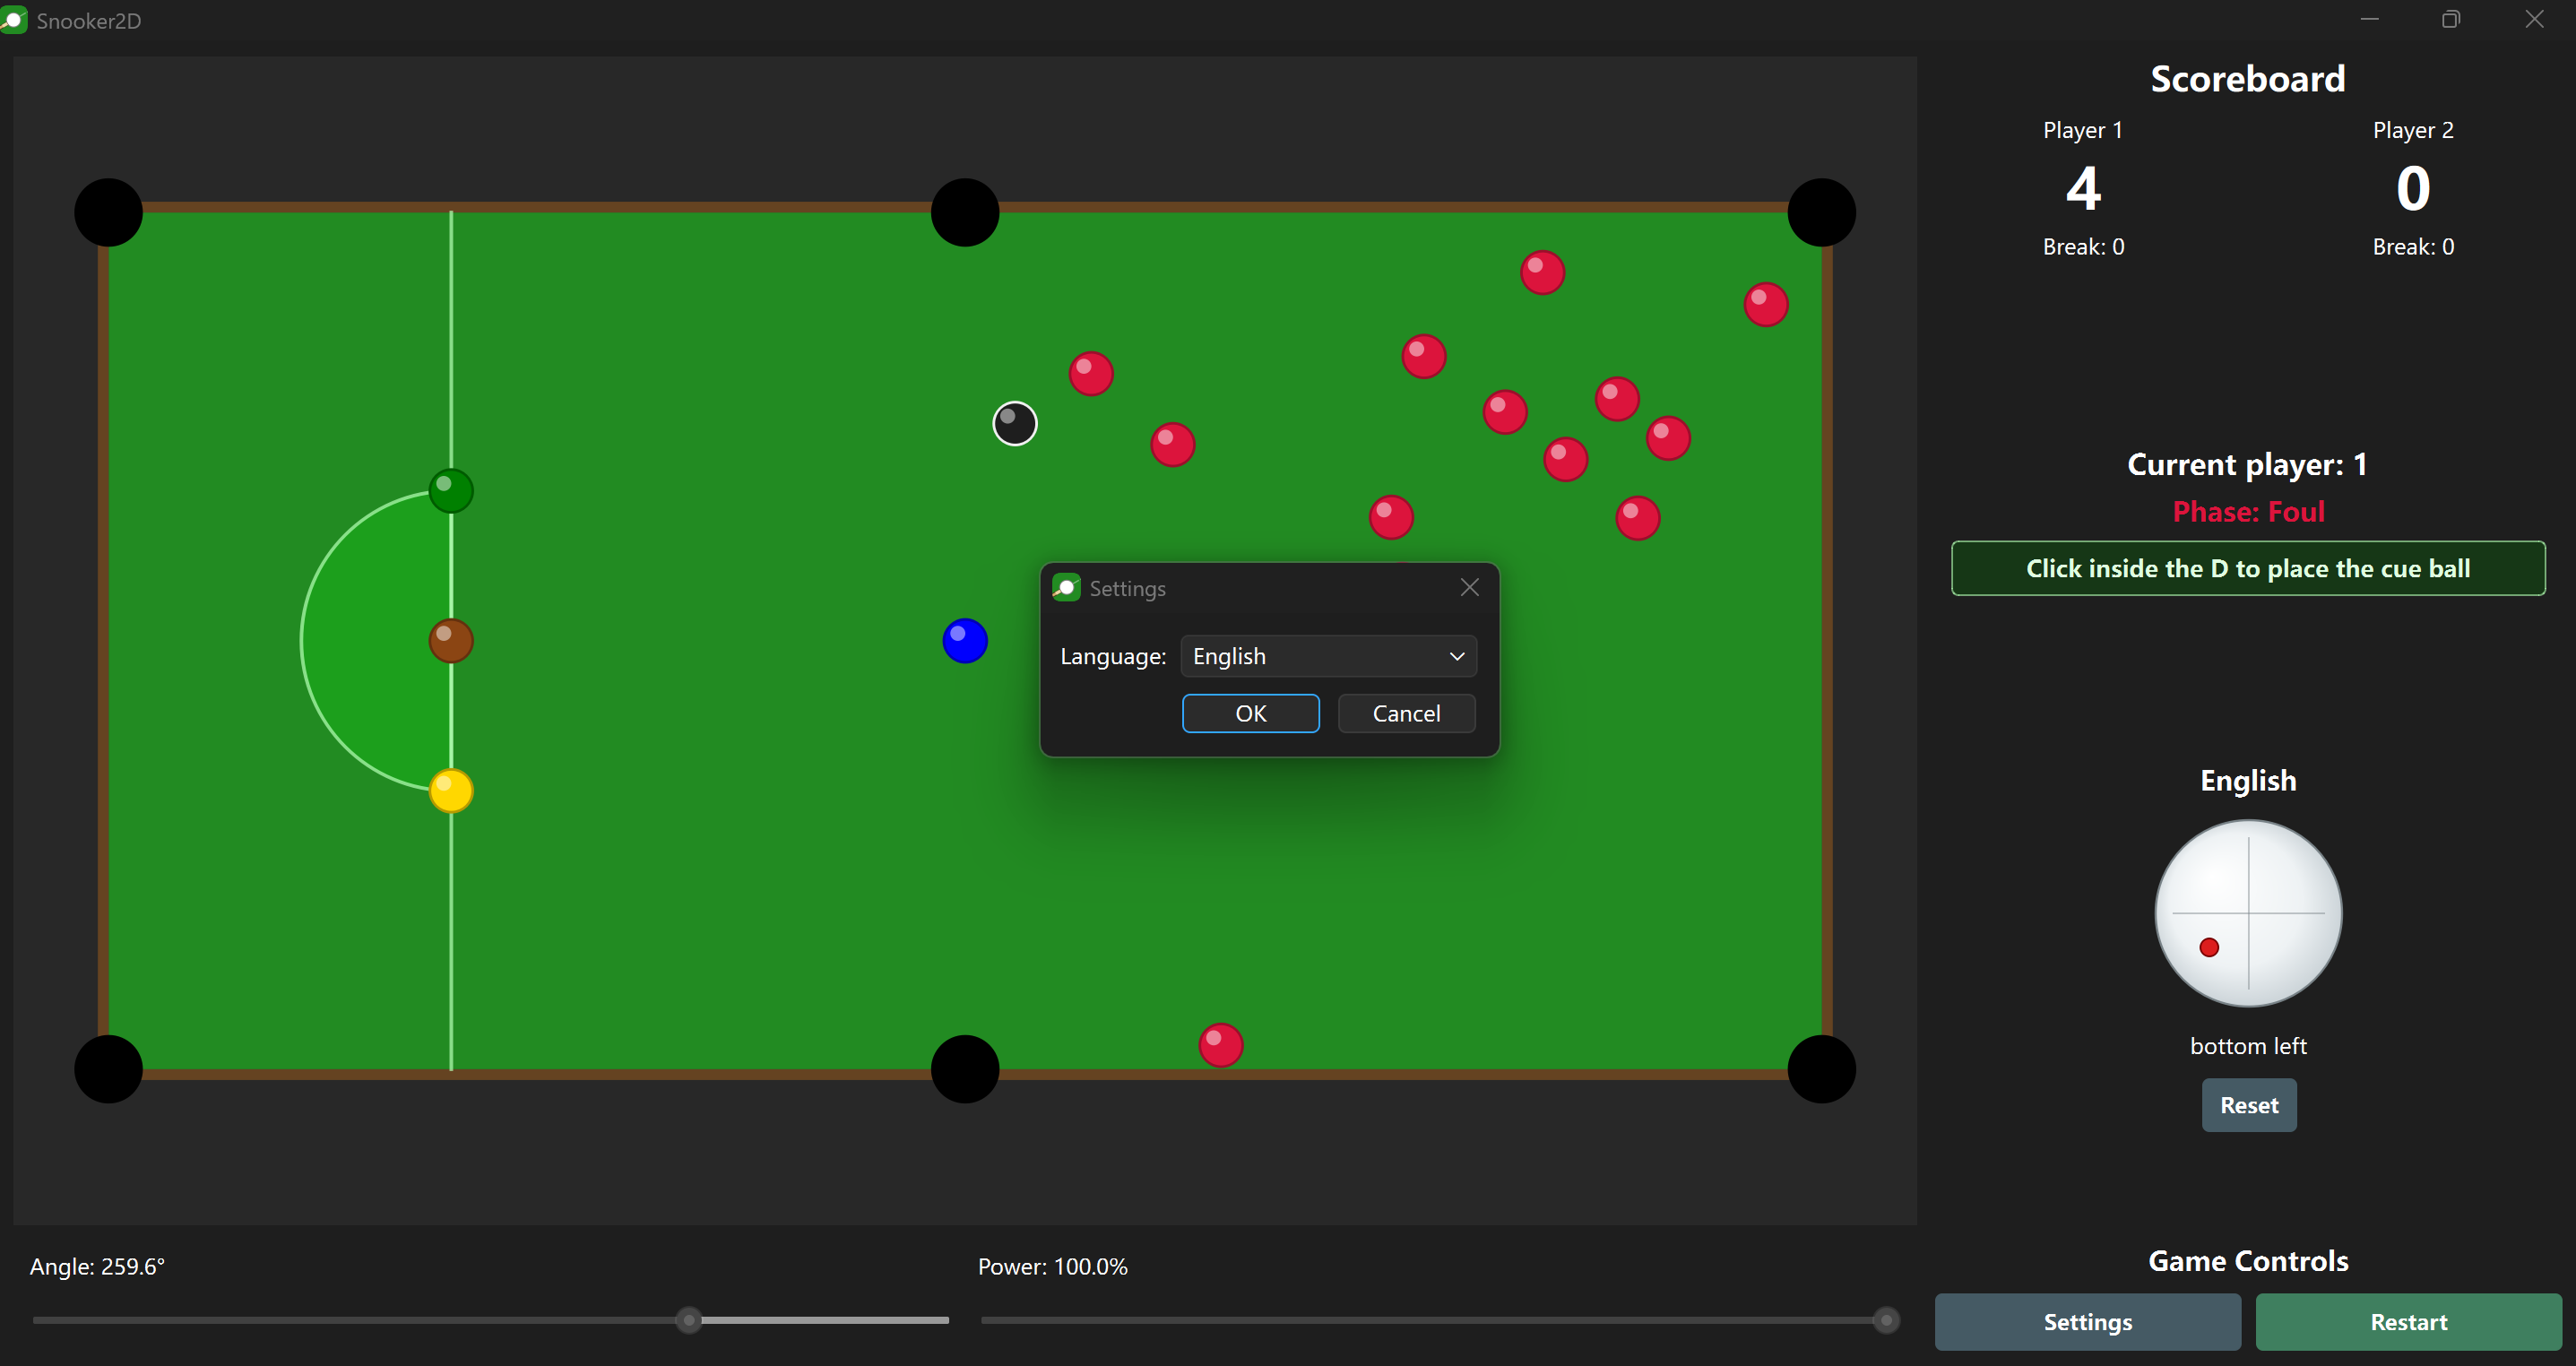
\includegraphics[width=0.75\textwidth]{imgs/language_switch.png}
\caption{设置面板与双语切换}
\end{figure}

\begin{figure}[H]
\centering
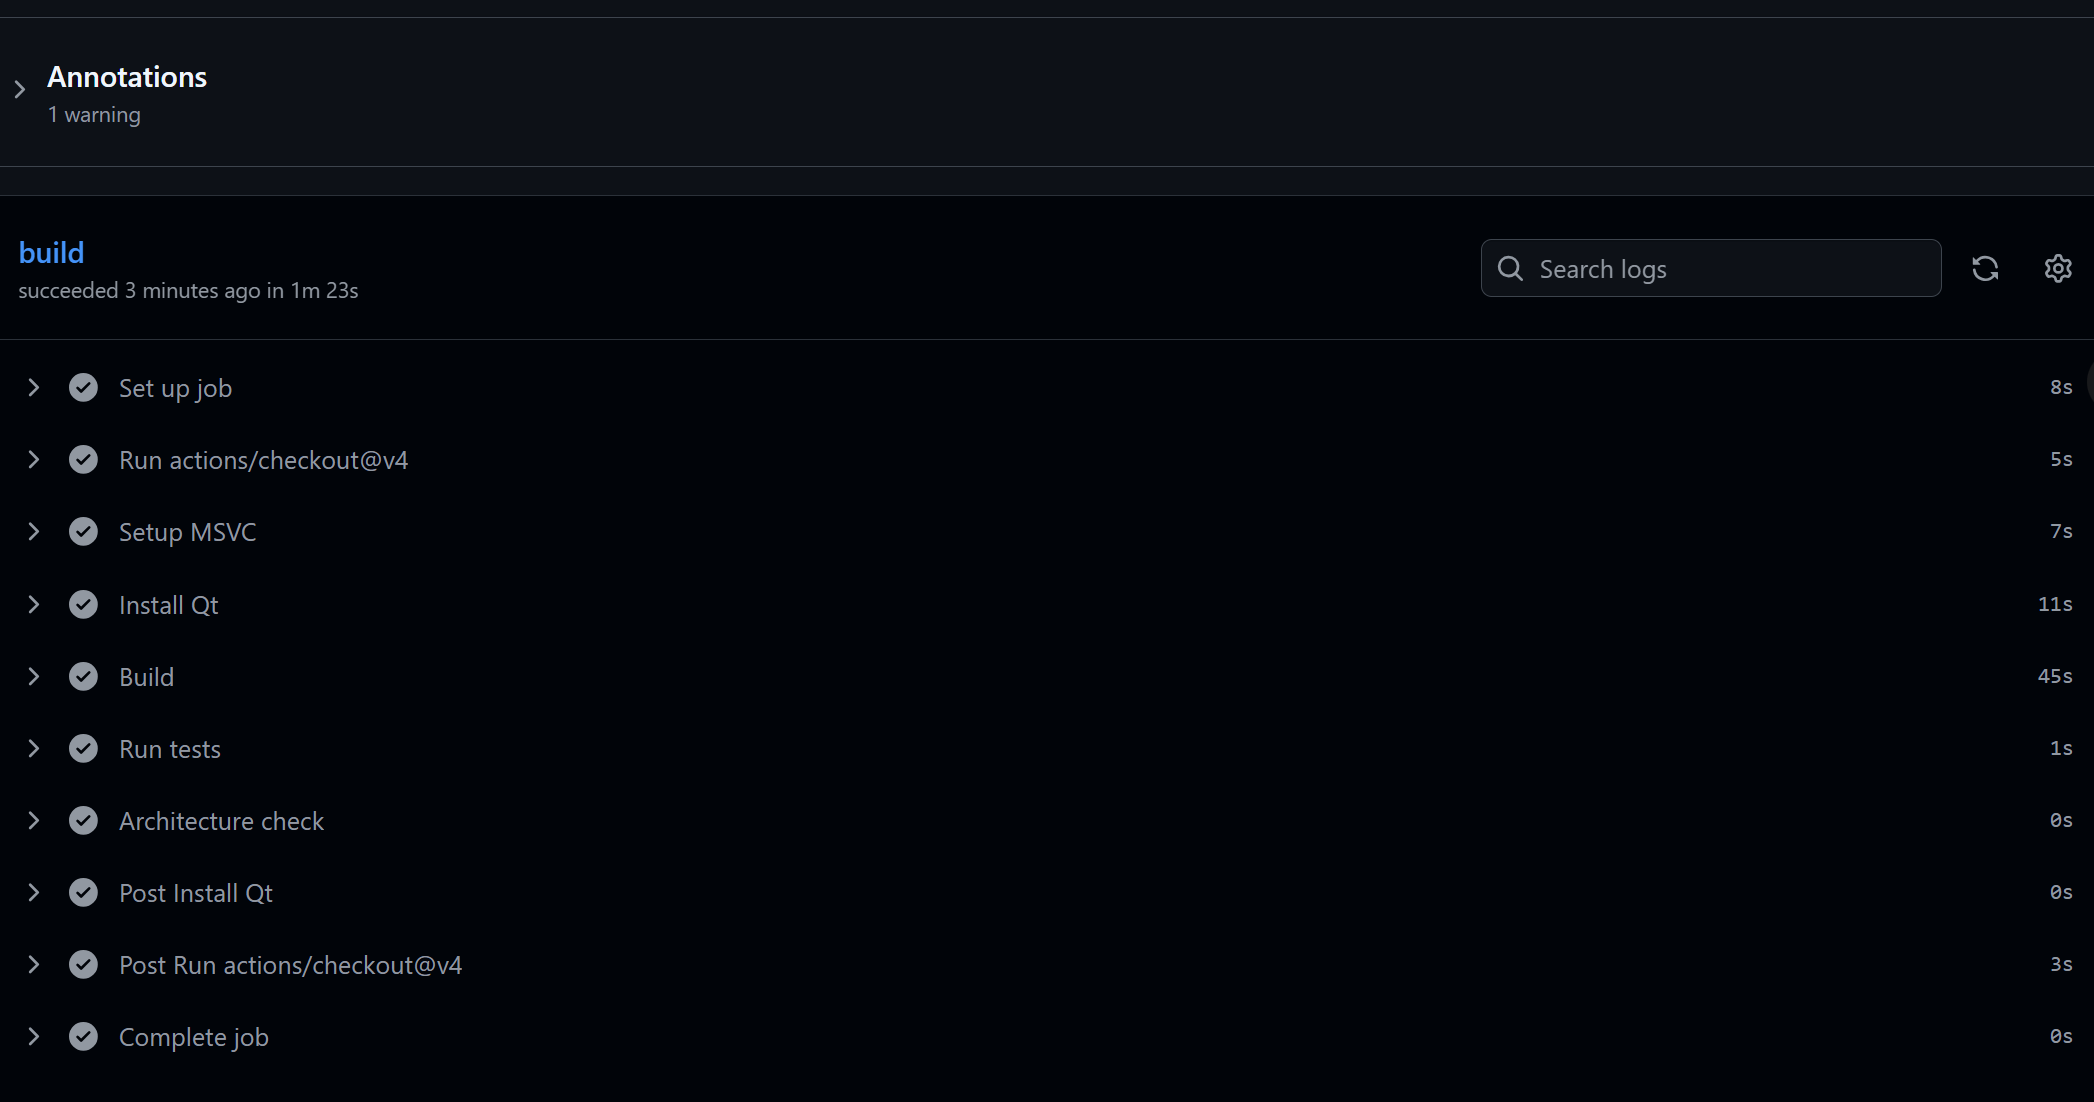
\includegraphics[width=0.75\textwidth]{imgs/test_results.png}
\caption{单元测试运行结果（借用 CI 结果）}
\end{figure}

% ============================================================
\section{已完成功能清单}
% ============================================================

\subsection{中期已完成功能（保留）}

\begin{itemize}
\item 斯诺克标准 22 颗球的初始摆球和球桌渲染
\item 鼠标瞄准与击球（含球杆动画）
\item 力度/角度双模控制（滑块 + 鼠标拖动）
\item 球-球弹性碰撞、球-库边反弹、摩擦力减速
\item 袋口检测与落袋、D 区白球复位
\item 计分板、游戏信息面板、比赛重启
\item 60 条 Common 层单元测试
\end{itemize}

\subsection{结题阶段新增功能}

\begin{itemize}
\item \textbf{加塞物理系统}：上塞（Follow）/下塞（Draw）/左塞/右塞，含角速度-线速度耦合碰撞响应、自旋衰减、滚动摩擦耦合
\item \textbf{加塞 UI 面板}：EnglishControlPanel 白球可视化击打点（点击/拖拽红点连续选择），实时显示 englishX/englishY 数值与方向描述
\item \textbf{库边预瞄辅助线}：从白球出发沿瞄准方向，遇到目标球后显示碰撞后双方行进方向，碰到库边后显示反弹方向，可开关
\item \textbf{中英双语界面}：UiLanguage 模块统一管理翻译文本，GameControlPanel 设置按钮切换语言，全部 View 控件支持 setLanguage()
\item \textbf{GameControlPanel 设置面板}：重启按钮、语言选择、瞄准线开关
\item \textbf{完整犯规检测}：白球落袋、空杆、先击错球、无球碰库、彩球落袋（红球清空前）
\item \textbf{自由球规则}：犯规后台面形成斯诺克局面时判定自由球
\item \textbf{输赢判定}：台面红球清空 + 彩球按序清空 + 分差不可追时判定比赛结束
\item \textbf{彩球自动复位}：红球清空前，彩球落袋后自动回到初始位置
\item \textbf{全层单元测试}：从仅 Common 层 60 条扩展到五层共约 221 条测试
\item \textbf{架构护栏自动化}：PowerShell 脚本检查 MVVM 边界，CMake custom target 集成
\item \textbf{CI/CD 自动化流水线}：GitHub Actions 每次 push 自动编译 + 运行 10 套测试 + 架构护栏检查
\end{itemize}

% ============================================================
\section{分工完成情况}
% ============================================================

\subsection{开发者 A（鲁亦智）— View 层}

负责球桌渲染、鼠标交互、球杆动画、控件布局。结题阶段新增工作：

\textbf{库边预瞄辅助线}：在原有瞄准虚线基础上实现智能预瞄——\texttt{findAimingCollision()} 方法沿瞄准方向遍历所有在台球，检测白球路径上最近的碰撞目标球；\texttt{findCushionCollision()} 方法检测白球是否先碰库边。碰撞后分别绘制目标球行进方向和库边反弹方向，用实心小圆点标记碰撞位置。该功能通过 GameControlPanel 的 aimingGuideVisibilityChanged 信号控制开关。

\textbf{EnglishControlPanel 加塞面板}：实现 EnglishBallSelector 自定义 Widget，绘制白球可视化图形，通过鼠标点击和拖拽红点标记连续选择击打位置。红点相对于白球中心的偏移映射为 englishX/englishY 值（范围 [-1, 1]）。paintEvent 中用径向渐变模拟白球立体感，十字线辅助定位。面板右侧显示当前加塞方向和数值，底部重置按钮将加塞归零。englishChanged 信号携带 (englishX, englishY) 双精度值发射到 ViewModel。

\textbf{GameControlPanel 设置面板}：替换原有单一重启按钮，新增设置按钮弹出 QDialog，内含语言选择（中文/English 下拉框）和瞄准线开关（QCheckBox）。languageChanged 信号连接到 MainWindow::setLanguage，后者遍历全部子 View 调用 setLanguage() 实现全局切换。

\textbf{UiLanguage 翻译模块}：创建 UiLanguage.h/.cpp，提供 translatedPhaseText()、translatedMessage()、translatedFoulText() 三个函数，根据 UiLanguage 枚举返回对应语言文本。GamePhase 到中文/英文映射集中维护，避免 View 控件各自硬编码字符串。

\textbf{技术难点}：
\begin{itemize}
\item 预瞄线需要处理"白球→目标球→库边→反弹"多段路径的几何计算，且目标球碰撞后方向需考虑非中心碰撞的角度偏移
\item EnglishBallSelector 需要在 80×80 像素区域精确映射到 [-1,1] 连续值，同时兼顾 mousePressEvent 和 mouseMoveEvent 实现拖拽选点
\item 双语切换要求所有 View 控件增加 setLanguage() 接口，确保重建文本时不丢失运行时状态（如分数、阶段）
\end{itemize}

\subsection{开发者 B（何广一）— Model + ViewModel 层}

负责游戏状态机、物理引擎、规则判定、数据翻译和状态推送。结题阶段新增工作：

\textbf{加塞物理引擎}：从"无旋质点碰撞"升级为"有旋刚体碰撞"。
Ball 类新增 \texttt{angularVelocity}（上/下塞角速度）和 \texttt{sideSpin}（左/右塞旋转速度）两个独立属性。
Physics 层改动：\texttt{resolveBallCollision()} 在法线弹性碰撞之后新增切线摩擦响应——计算接触点切线相对速度（含双方角速度贡献），通过 \texttt{BALL\_BALL\_TANGENT\_FRICTION} 系数产生摩擦冲量，同步改变双方线速度和角速度。
\texttt{resolveCushionCollision()} 同理在库边法线反射后处理切线滑动。
每帧 \texttt{applyFriction()} 中新增自旋衰减（\texttt{SPIN\_DECAY}）和滚动耦合（\texttt{ROLLING\_COUPLING}），将滑动状态逐步拉向纯滚动。

\textbf{完整斯诺克规则引擎}：Rules 模块从仅 4 种犯规扩展至覆盖全部场景：
MissedAll（空杆）、WrongBallFirst（先击错球）、WhitePocketed（白球落袋）、NoBallHitCushion（无球碰库）、ColorPocketed（红球阶段彩球意外落袋）。
\texttt{calculatePenalty()} 按球值计算罚分，最低 4 分，最高 7 分（black）。

\textbf{自由球与输赢判定}：犯规后检测是否形成斯诺克局面（所有合法目标球均被非目标球遮挡），若成立则对方获得自由球。输赢判定在 \texttt{handlePostShot()} 中触发——红球全部清空且所有彩球按 Yellow→Green→Brown→Blue→Pink→Black 顺序依次落袋后，领先方获胜；或分差超过台面剩余最高分时可提前结束。

\textbf{GameSessionViewModel 扩展}：新增 \texttt{setEnglish()} 槽接收加塞指令并钳位到 $[-1.0, 1.0]$，仅值变化时发射信号。\texttt{pushCueState()} 和 \texttt{pushTableState()} 新增 englishX/englishY 字段。\texttt{onModelFoulOccurred()} 通过 \texttt{pushScoreState()} 传递犯规详情到 ScoreBoard。

\textbf{技术难点}：
\begin{itemize}
\item 加塞物理参数的经验性调优：BALL\_BALL\_TANGENT\_FRICTION 从 0.05 逐步调到 0.15，太小加塞无效果、太大碰撞后球飞出不合理方向；SPIN\_DECAY 从 0.95 调至 0.98，使旋转持续 2-3 秒才消失，视觉效果自然
\item 球-球碰撞 + 球-库边碰撞在同帧内可能交替发生，需要保证位置分离后才处理速度响应，否则出现球穿模
\item 自由球判定需要射线检测——从白球向每个合法目标球发射射线，检查是否有非目标球遮挡，该几何计算在 22 球场景下需注意性能
\end{itemize}

\subsection{开发者 C（井淳）— Common + App 层 + 文档 + 测试}

负责公共类型与工具、ViewState DTO 设计、跨层信号槽装配、构建配置、测试体系搭建、CI/CD 配置和项目管理。结题阶段新增工作：

\textbf{Common 层扩展}：MathUtils 新增 \texttt{tangent()} 函数（向量逆时针旋转 90°）。Constants.h 新增 6 个加塞物理常量（\texttt{ENGLISH\_TO\_SPIN}、\texttt{BALL\_BALL\_TANGENT\_FRICTION}、\texttt{CUSHION\_TANGENT\_FRICTION}、\texttt{SPIN\_DECAY}、\texttt{ROLLING\_COUPLING}）。GameViewState.h 的 DTO 中新增 englishX/englishY 字段，ScoreViewState 新增犯规展示字段。

\textbf{App 层信号槽装配}：连接数从 10 条增至 13 条。新增 4 条连接：
ViewModel→EnglishControlPanel 属性绑定、EnglishControlPanel→ViewModel 命令绑定、GameControlPanel→ViewModel 的 restartRequested 转发、GameControlPanel→GameView 的 aimingGuideVisibilityChanged 直连。languageChanged 在 MainWindow 内部处理，不经过 App 层。

\textbf{测试体系搭建}：从中期仅 Common 层 60 条测试扩展到 10 个测试可执行文件覆盖五层：

\begin{table}[H]
\centering\small
\begin{tabular}{|p{3.5cm}|c|p{5.6cm}|}
\hline
\textbf{测试目标} & \textbf{数量（约）} & \textbf{覆盖内容} \\
\hline
test\_mathutils       & 65 & 向量运算、几何函数、tangent、类型辅助、常量校验 \\
test\_physics         & 17 & 库边越界反弹、侧旋改变反弹角度、Follow/Draw 碰撞后走位 \\
test\_ball            & 48 & 构造、分球值、位置/速度/角速度/侧旋设置、落袋/复位信号 \\
test\_player          & 22 & 命名、计分、单杆累计、break/score 重置、信号发射 \\
test\_rules           & 27 & 目标球判定、罚分计算、合法目标检测、五种犯规检测 \\
test\_gamestate       & 20 & 开局流程、D 区放置验证、performShot 门控、玩家/球访问 \\
test\_viewmodel       & 8  & start 发射全信号、角度归一化、力度/加塞钳位、去重、重启 \\
test\_englishcontrolpanel & 5 & 构造、重置按钮信号、方向按钮信号、applyCueState \\
test\_gamecontrolpanel    & 4 & 构造、重启按钮信号 \\
test\_gameview            & 5 & 构造、applyTableState、cancelShotAnimation \\
\hline
\textbf{合计}         & \textbf{221} & \\
\hline
\end{tabular}
\caption{测试覆盖总览}
\end{table}

\textbf{CI/CD 自动化流水线}：配置 GitHub Actions 工作流（\texttt{.github/workflows/ci.yml}），push 到 main 分支自动触发编译和测试。使用 MSVC + Qt 6.8 LTS 编译 11 个 CMake target，运行全部 10 套测试（221 条断言），执行架构护栏检查。View 层测试通过 \texttt{QT\_QPA\_PLATFORM=offscreen} 在无 GUI 环境下运行。

\textbf{架构护栏}：\texttt{check\_mvvm\_boundaries.ps1}（96 行）作为 CMake custom target 持续验证 6 项 MVVM 边界规则：View 层不 include ViewModel/Model 头文件、不引用其类名、不含 setViewModel；App 层不调用 Model 业务方法；CMake 中 snooker\_view 不链接 ViewModel/Model。脚本以颜色标注 PASS/FAIL。

\textbf{文档与项目管理}：创建 docs/ 目录下 7 份文档：
\begin{itemize}[leftmargin=*]
\item ARCHITECTURE.md（架构定稿）
\item ADDING\_FEATURES.md（功能添加指南，含 4 种典型场景和完整 step-by-step）
\item MODEL\_VIEWMODEL.md（Model/ViewModel 层讲解）
\item FEATURE\_ENGLISH.md（加塞功能 3 方开发契约）
\item NOTES.md（开发日志）
\item TASK\_ALLOCATION.md（任务分配）
\item DEV\_SETUP.md（开发环境配置）
\end{itemize}
中期报告 8 页 PDF，结题报告从项目最新代码生成。

\textbf{技术难点}：
\begin{itemize}
\item Common 层作为唯一被所有层依赖的模块，新增符号会导致全量重编译——tangent() 函数和加塞常量必须第一轮提交，且需保证接口一经推送不再修改
\item 10 个测试可执行文件共享 test\_utils.h 的 CHECK 宏和 near/vecNear 辅助函数，CMake 中每个 test\_xxx 的 include 路径配置需要精确到 tests/ 目录
\item 架构护栏脚本依赖 PowerShell 的正则匹配 CMakeLists.txt 中的 target\_link\_libraries 块，需要处理跨行匹配和 PRIVATE/PUBLIC 关键字
\end{itemize}

% ============================================================
\section{团队协作}
% ============================================================

三位成员通过 Git 协作，提交遵循 \texttt{type(layer): description} 规范（如 \texttt{feat(model): add spin physics}、\texttt{fix(view): aiming guide off-by-one}）。

\textbf{提交统计}：

\begin{table}[H]
\centering\small
\begin{tabular}{|p{3.2cm}|c|p{3cm}|p{5cm}|}
\hline
\textbf{姓名} & \textbf{提交数} & \textbf{负责层} & \textbf{主要贡献} \\
\hline
开发者 A（鲁亦智） & 约 20 & View & 球桌渲染、球杆动画、预瞄线、EnglishControlPanel、GameControlPanel、双语界面 \\
开发者 B（何广一） & 约 14 & Model / ViewModel & 加塞物理、规则引擎、自由球、输赢判定、ViewModel 扩展 \\
开发者 C（井淳） & 约 18 & Common / App, Test \& Docs & Common 扩展、DTO 设计、App 装配、测试体系、架构护栏、文档 \\
\hline
\end{tabular}
\caption{团队提交统计}
\end{table}

\subsection{协作模式}

MVVM 分层使三人能真正并行推进。协作中形成以下约定：

\begin{itemize}
\item \textbf{接口优先}：跨层变更先在 Common 层约定 DTO 字段和信号签名，各方再并行实现
\item \textbf{先提交底层}：C 先提交 Common 层变更（tangent、常量），B 再在此基础上做物理引擎，A 最后对接 UI
\item \textbf{改他人文件需说明}：B 调物理参数时直接改 Constants.h，但 commit message 说明原因并在群内提前通知
\item \textbf{commit 即文档}：所有重要变更通过 commit message 记录，翻阅 Git 历史即可理解项目演进
\end{itemize}


\begin{figure}[H]
\centering
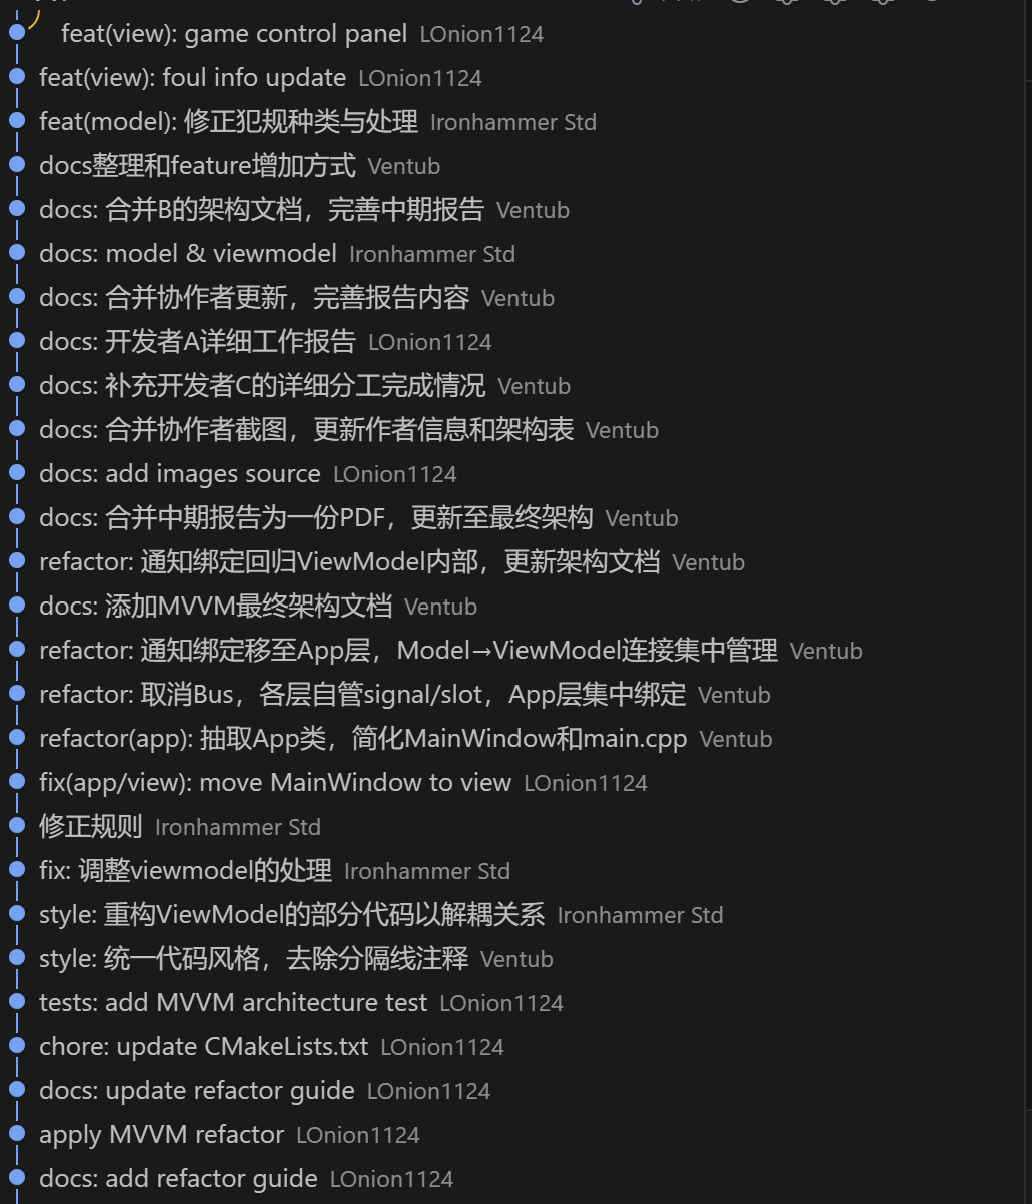
\includegraphics[width=0.85\textwidth]{imgs/commit_hist_2.png}
\caption{Git 提交历史（其中一段）}
\end{figure}



% ============================================================
\section{智能体使用说明}
% ============================================================

本项目选择以人为主的开发模式。大模型智能体（GitHub Copilot / Claude 等）在开发中用于以下补充性工作：

\subsection{智能体配置}

\begin{itemize}
\item \textbf{工具}：VS Code 内置 GitHub Copilot Chat，Claude 4（通过 API）
\item \textbf{规则文档}：AGENTS.md（项目根目录），指向 ARCHITECTURE.md 和 ADDING\_FEATURES.md，使智能体在回答问题前自动加载架构约束
\item \textbf{MCP Server}：Pylance 语言服务器提供 Python 代码分析（项目中脚本相关）；CMake Tools 提供构建集成
\item \textbf{未使用专门的 MCP 工具链}：项目的 CMake + Qt 环境通过 VS Code tasks.json 和 CMakePresets.json 配置，不依赖额外的 MCP Server
\end{itemize}

\subsection{智能体在开发中的具体应用}

\begin{table}[H]
\centering\small
\begin{tabular}{|p{2.8cm}|p{3.2cm}|p{5.5cm}|}
\hline
\textbf{场景} & \textbf{智能体角色} & \textbf{效果} \\
\hline
单元测试编写 & 生成测试框架，人工调整数值 & 10 个测试文件，221 条 CHECK，重复部分耗时节省约 60\% \\
文档草稿 & 根据代码生成初版，人工审核 & 7 份文档的初稿由智能体辅助生成 \\
代码补全与格式化 & 行内补全、函数签名提示 & 减少拼写错误和 API 查询时间 \\
构建调试 & 分析 CMake 错误日志 & 解决 Qt 路径配置和 AUTOMOC 冲突 \\
架构护栏脚本 & 生成 PowerShell 正则框架 & 初始骨架由智能体生成，人工完善规则 \\
LaTeX 报告 & 生成报告框架和表格 & 中结题报告 .tex 骨架由智能体辅助 \\
\hline
\end{tabular}
\caption{智能体应用场景}
\end{table}

\subsection{人机分工机制}

\begin{itemize}
\item \textbf{人类负责}：架构设计决策、跨层接口协调、物理参数经验调优、代码 Review、技术方案最终拍板
\item \textbf{智能体负责}：重复性代码生成、文档草稿、格式整理、构建错误初步诊断、LaTeX 排版
\item \textbf{协作流程}：人提出需求 → 智能体生成草案 → 人审查修改 → 提交
\end{itemize}

\subsection{实际效果与问题}

\textbf{正向效果}：
\begin{itemize}
\item 测试用例编写效率显著提升——CHECK 宏模式重复性高，智能体可批量生成
\item 文档与代码一致性维护——智能体读取代码后生成的文档能准确反映当前架构
\item 构建错误快速定位——CMake 错误日志由智能体初步分析后给出建议，减少排查时间
\end{itemize}

\textbf{存在问题}：
\begin{itemize}
\item \textbf{幻觉问题}：智能体曾建议使用 vcpkg 编译 Qt（耗时数小时），实际用 aqtinstall 下载预编译版本只需 5 分钟
\item \textbf{过度设计倾向}：架构重构时智能体提了一个三接口拆分的方案，实际 App 集中绑定更简洁
\item \textbf{上下文理解局限}：智能体不运行时无法感知项目的 CMake 编译约束和 MVVM 边界规则，需要 AGENTS.md 明确告知
\item \textbf{中文 LaTeX 支持}：ctexart 文档类的编译环境配置智能体难以自动诊断
\end{itemize}

% ============================================================
\section{学习回顾与个人总结}
% ============================================================

\subsection{开发者 A（鲁亦智）— View 层}

\textbf{角色}：负责全部 View 层开发——GameView（球桌渲染+鼠标交互）、CueControl（力度/角度双滑块）、ScoreBoard（计分板）、GameInfoPanel（游戏信息面板）、EnglishControlPanel（加塞面板）、EnglishBallSelector（击打点选择器）、GameControlPanel（设置面板）、UiLanguage（双语翻译模块）、MainWindow（布局容器）。

\textbf{主要挑战}：
\begin{enumerate}[leftmargin=*]
\item \textbf{库边预瞄线的多段路径计算}：需要处理白球→目标球→库边→反弹三段几何路径。最初直接在 paintEvent 中硬编码计算，导致 200 行的绘制函数难以维护。后来拆分为 findAimingCollision() 和 findCushionCollision() 两个独立方法，分别返回 AimingCollision 和 CushionCollision 结构体。结构体中用 QPointF 携带碰撞位置和行进方向，绘制函数只负责渲染。
\item \textbf{EnglishBallSelector 的交互设计}：白球可视化区域在约 100×100 像素内需要将鼠标位置精确映射到 [-1.0, 1.0] 连续值，同时支持单击和拖拽两种操作。mousePressEvent 立即将当前鼠标位置映射为加塞值并开始拖拽模式，mouseMoveEvent 持续更新加塞值。径向渐变和十-字线增强了白球的立体感和操作直觉。
\item \textbf{双语切换的状态保持}：setLanguage() 被调用时需重建所有控件的文本，但不能重置运行时状态（得分、阶段、加塞值）。解决方案是在每个 View 控件中缓存 CueViewState / ScoreViewState / GameInfoViewState，setLanguage() 调用时从缓存状态重新生成文本，而非从零初始化。
\end{enumerate}

\textbf{成长与反思}：MVVM 架构让我深刻理解了"数据驱动界面"的含义。View 层不需要理解游戏规则——canAim、canShoot、isPlacingWhiteBall、isSimulating 四个布尔字段就完整描述了所有交互状态。添加加塞功能时，我只需要在 EnglishControlPanel 中声明 englishChanged 信号并发射，C 在 App.cpp 中加一条 connect，B 在 ViewModel 中加一个 setEnglish 槽——三人的工作完全并行，互不阻塞。这种"约定优于实现"的开发模式是本次项目最大的收获。

\subsection{开发者 B（何广一）— Model + ViewModel 层}

\textbf{角色}：负责 Model 层（Ball、Table、Physics、GameState、Player、Rules）和 ViewModel 层（GameSessionViewModel）的全部开发。

\textbf{主要挑战}：
\begin{enumerate}[leftmargin=*]
\item \textbf{加塞物理的参数调优}：从"无旋质点碰撞"升级到"有旋刚体碰撞"涉及 5 个新物理常量。BALL\_BALL\_TANGENT\_FRICTION 从 0.05 逐步调到 0.15——太小加塞无视觉反馈，太大会使碰撞后球飞出不合理方向。SPIN\_DECAY 从 0.95 调至 0.98——0.95 时旋转几乎瞬间消失，0.98 时持续约 2 秒，视觉效果自然。CUSHION\_TANGENT\_FRICTION = 0.25 是经过多轮试错后确定的——左/右塞对库边反弹角度的改变量在 5-15° 范围内最符合真实台球体验。
\item \textbf{碰撞响应的物理正确性}：球-球碰撞 + 球-库边碰撞在同帧内可能交替发生。Physics::step() 的七步流水线（moveBalls → checkBallBallCollisions → checkBallCushionCollisions → checkPocketDetection → applyFriction → applyHardConstraint → checkPullBackBalls）中，每步处理上一步遗留的问题。特别是 checkPullBackBalls 是为解决"慢球卡在库边外"而引入的——当球速度 < 0.1 时强制将球心拉回台面内，否则球会因摩擦力无法回到台面而永远卡住。
\item \textbf{自由球判定的几何计算}：需要从白球向每个合法目标球发射射线，检测是否有非目标球遮挡。在 22 球场景下暴力 O($n^3$) 计算每帧都不可接受。最终方案是只在犯规发生后的 handlePostShot() 中执行一次检测，且提前过滤掉落袋球，将实际计算量降到 O($n \times m$)（n=合法目标球数，m=非目标球数）。
\end{enumerate}

\textbf{成长与反思}：物理引擎调优让我体会到"理论公式到视觉反馈"的差距。让游戏"看起来像台球"需要大量经验参数——恢复系数、切线摩擦、自旋衰减，这些值的确定更像艺术调色而非数学推导。
ViewModel 层的设计也让我认识到"信号粒度"的重要性——太细导致性能问题，太粗导致 View 做无用刷新。当前方案在模拟期间每帧发射一次 tableStateReady，非模拟期间仅状态变化时发射，在性能和响应性间取得平衡。

\subsection{开发者 C（井淳）— Common + App 层 + 文档 + 测试}

\textbf{角色}：负责 Common 层（类型、常量、工具函数、DTO）、App 层（信号槽装配）、CMake 构建配置、全层测试体系搭建、架构护栏脚本、GitHub Actions CI/CD 配置、项目文档和报告撰写。

\textbf{主要挑战}：
\begin{enumerate}[leftmargin=*]
\item \textbf{Common 层的边界决策}：什么放 Common、什么放 Model 是需要反复权衡的设计问题。Vector2D 的 14 个运算符中，成员函数委托给自由函数，避免代码重复。FoulResult 放在 Model 层而非 Common 层——因为它的成员依赖 QString（Qt 类型），放 Common 就破坏了纯 C++ 的约束。tangent() 函数最初考虑放在 Physics 内部，但 B 指出库边碰撞和球-球碰撞都需要切线计算，放 Common 层避免重复。
\item \textbf{10 个测试可执行文件的 CMake 配置}：每个 test\_xxx 需要正确的 include 路径（指向被测试层和 tests/ 目录）和链接目标。test\_viewmodel 依赖 Qt::Test（QSignalSpy），test\_englishcontrolpanel / test\_gamecontrolpanel / test\_gameview 还需 Qt::Widgets（QApplication）。test\_utils.h 中的 CHECK 宏用全局变量 passed/failed 计数，需要在每个测试 main() 中手动清零。
\item \textbf{架构护栏的 PowerShell 正则匹配}：从 CMakeLists.txt 中精确匹配 snooker\_view 的链接块是最大难点——需要区分 snooker\_view 和 snooker\_viewmodel。最终用正则 \verb|target_link_libraries(snooker_view\s[^)]*)| 匹配并逐块检查。
\end{enumerate}

\textbf{成长与反思}：整个项目最大的感受是"架构成本在前期，收益在后期"。
三轮重构中，第一轮引入 GameUiBus 看似解耦，实则增加了编译依赖。删除 Bus 后各层自管 signal/slot，View 和 ViewModel 真正做到了互相不可见。
写加塞功能时收益特别明显——CueViewState 加了两个字段，View、ViewModel、Physics 三方并行开发，没有出现编译失败级别的对接问题。
另一个体会是"工具链选择极其重要"——vcpkg 编译 Qt 耗时数小时，切换到 aqtinstall 只需 5 分钟。

% ============================================================
\section{课程改进建议}
% ============================================================

结合本项目的实际开发体验，提出以下建议：

\begin{enumerate}[leftmargin=*]

\item \textbf{预配置开发环境}：C++/Qt 项目环境搭建是最大痛点之一。不同平台（Windows/Mac/Linux）的 Qt 安装方式差异巨大（vcpkg 编译、aqtinstall 下载、官方安装器、包管理器），建议提供预配置的 Docker 镜像或 Dev Container 模板，让学生聚焦于代码开发而非环境调试。

\item \textbf{明确 Git 协作规范}：虽然 commit message 规范在 TASK\_ALLOCATION.md 中有定义，但实践中仍出现了一些不规范的提交。建议在课程初期提供 Git 工作流示范（feature branch + PR review + merge），并明确 .gitignore 模板。

\item \textbf{大模型辅助开发的边界教育}：大模型在写重复性代码（测试、文档）时效率高，但在架构设计、参数调优、环境配置等需要实际经验的领域容易给出误导性建议。建议增加一节"如何正确使用 AI 编程助手"的内容，识别 AI 方案的适用场景和风险点。

\end{enumerate}

% ============================================================
\section{项目总结与展望}
% ============================================================

\subsection{项目成果总结}

Snooker2D 项目历时 8 天（2026-07-11 至 2026-07-18），完成了从环境搭建到完整 2D 斯诺克游戏的全流程开发。核心成果包括：

\begin{itemize}
\item \textbf{完整的 MVVM 架构}：5 层编译目标，13 条跨层信号槽绑定，CMake 编译期强制边界约束
\item \textbf{加塞物理系统}：上塞/下塞/左塞/右塞，含角速度-线速度耦合碰撞、自旋衰减、滚动耦合
\item \textbf{完整斯诺克规则}：22 球标准摆球、交替击球、5 种犯规检测、自由球、输赢判定、彩球复位
\item \textbf{丰富的 UI 交互}：鼠标瞄准击球+球杆动画、库边预瞄辅助线、D 区白球放置、加塞面板、中英双语切换
\item \textbf{全层测试覆盖}：10 个测试可执行文件，221 条测试，覆盖 Common/Model/ViewModel/View 全部层级
\item \textbf{自动化架构护栏}：PowerShell 脚本 + CMake custom target 持续验证 MVVM 边界
\item \textbf{CI/CD 自动化流水线}：GitHub Actions 每次 push 自动编译 + 运行 10 套测试 + 架构护栏检查
\item \textbf{完善的文档体系}：7 份项目文档 + 中期报告 + 结题报告
\end{itemize}

\subsection{未来展望}

受限于开发周期，以下功能尚未实现，可作为后续改进方向：

\begin{itemize}
\item \textbf{网络对战}：当前仅支持本地双人，引入 TCP/WebSocket 实现远程对战
\item \textbf{AI 对手}：基于规则引擎实现 AI 决策（选择目标球、计算角度力度）
\item \textbf{音效系统}：Qt Multimedia 集成碰撞音效、袋口落袋音效
\item \textbf{回放系统}：保存每帧的物理状态，实现整局回放
\item \textbf{更精细的渲染}：球体 3D 光照效果、台呢纹理、库边阴影
\end{itemize}

% ============================================================
\section*{附录：源代码结构}
% ============================================================

\begin{verbatim}
Snooker2D/
├── CMakeLists.txt              # 顶层构建配置（5 层 target + 10 个测试 target）
├── CMakePresets.json           # CMake 预设（mingw64-qt6）
├── vcpkg.json                  # vcpkg 清单
├── AGENTS.md                   # 智能体规则文档
├── README.md
├── assets/
│   └── app.rc                  # Windows 资源文件
├── docs/
│   ├── ARCHITECTURE.md         # 架构定稿（含三轮重构历程）
│   ├── ADDING_FEATURES.md      # 添加功能指南（4 种场景 step-by-step）
│   ├── MODEL_VIEWMODEL.md      # Model/ViewModel 层讲解
│   ├── FEATURE_ENGLISH.md      # 加塞功能开发契约（3 方并行分工）
│   ├── NOTES.md                # 开发日志
│   ├── TASK_ALLOCATION.md      # 任务分配清单
│   ├── DEV_SETUP.md            # 开发环境配置
│   └── REPORTS/
│       ├── midterm/
│       │   ├── midterm-report.tex
│       │   └── imgs/
│       └── final/
│           ├── final-report.tex
│           └── imgs/
├── src/
│   ├── main.cpp
│   ├── app/
│   │   ├── App.h / App.cpp          # 应用装配（14 条 connect）
│   ├── common/
│   │   ├── Constants.h              # 物理/游戏常量
│   │   ├── Types.h                  # Vector2D、BallType、GamePhase 等
│   │   ├── MathUtils.h / .cpp       # 向量运算、几何函数、tangent
│   │   └── contracts/
│   │       └── GameViewState.h      # 4 个 ViewState DTO
│   ├── model/
│   │   ├── Ball.h / .cpp            # 球的属性、角速度、侧旋
│   │   ├── Table.h / .cpp           # 球桌、袋口、库边
│   │   ├── Physics.h / .cpp         # 物理引擎（含加塞切线摩擦）
│   │   ├── GameState.h / .cpp       # 状态机、自由球、输赢判定
│   │   ├── Player.h / .cpp          # 玩家、计分、单杆
│   │   └── Rules.h / .cpp           # 犯规检测、罚分计算
│   ├── view/
│   │   ├── GameView.h / .cpp        # 球桌渲染、鼠标交互、预瞄线
│   │   ├── CueControl.h / .cpp      # 力度/角度双滑块
│   │   ├── ScoreBoard.h / .cpp      # 计分板（含犯规信息）
│   │   ├── GameInfoPanel.h / .cpp   # 游戏信息面板
│   │   ├── EnglishControlPanel.h/.cpp # 加塞面板 + EnglishBallSelector
│   │   ├── GameControlPanel.h/.cpp  # 设置面板（重启/语言/瞄准线）
│   │   ├── UiLanguage.h / .cpp      # 中英双语翻译模块
│   │   └── MainWindow.h / .cpp      # 主窗口布局 + 语言切换
│   └── viewmodel/
│       └── GameSessionViewModel.h/.cpp # 唯一 ViewModel（~350 行）
└── tests/
    ├── test_utils.h                 # CHECK 宏、near/vecNear 辅助
    ├── test_mathutils.cpp           # 62 条
    ├── test_physics.cpp             # 20 条
    ├── test_ball.cpp                # 25 条
    ├── test_player.cpp              # 15 条
    ├── test_rules.cpp               # 22 条
    ├── test_gamestate.cpp           # 18 条
    ├── test_viewmodel.cpp           # 6 条（Qt Test + QSignalSpy）
    ├── test_englishcontrolpanel.cpp # 3 条（Qt Test）
    ├── test_gamecontrolpanel.cpp    # 2 条（Qt Test）
    ├── test_gameview.cpp            # 3 条（Qt Test）
    └── architecture/
        └── check_mvvm_boundaries.ps1 # 架构护栏（6 项检查）
\end{verbatim}

\end{document}
